\todo{Einstein puzzle as a running example? [T] if we call it holy zebra, makes sense to use Zebra as running example}



\ourtool takes as input a set of natural language sentences (from hereon referred to as ``clues'') and (optionally) domain information (names/values of the different entities in the problem domain).
In typical logic grid puzzles, this domain information is present in the grid. 
For some puzzles, domain information is not required; a prototypical example is Einstein's Zebra puzzle, which ends with the question ``who owns the zebra?'', while the puzzle can be solved without knowledge of the fact that there is a zebra in the first place. 
As we will detail below, for some puzzles, especially those with numeric values involved, this domain information is crucial to solving them. 

\ourtool then does this and this and that ... 

Figure \ref{fig:overview} contains an overview of the different components of the system.

\begin{figure*}
\centering
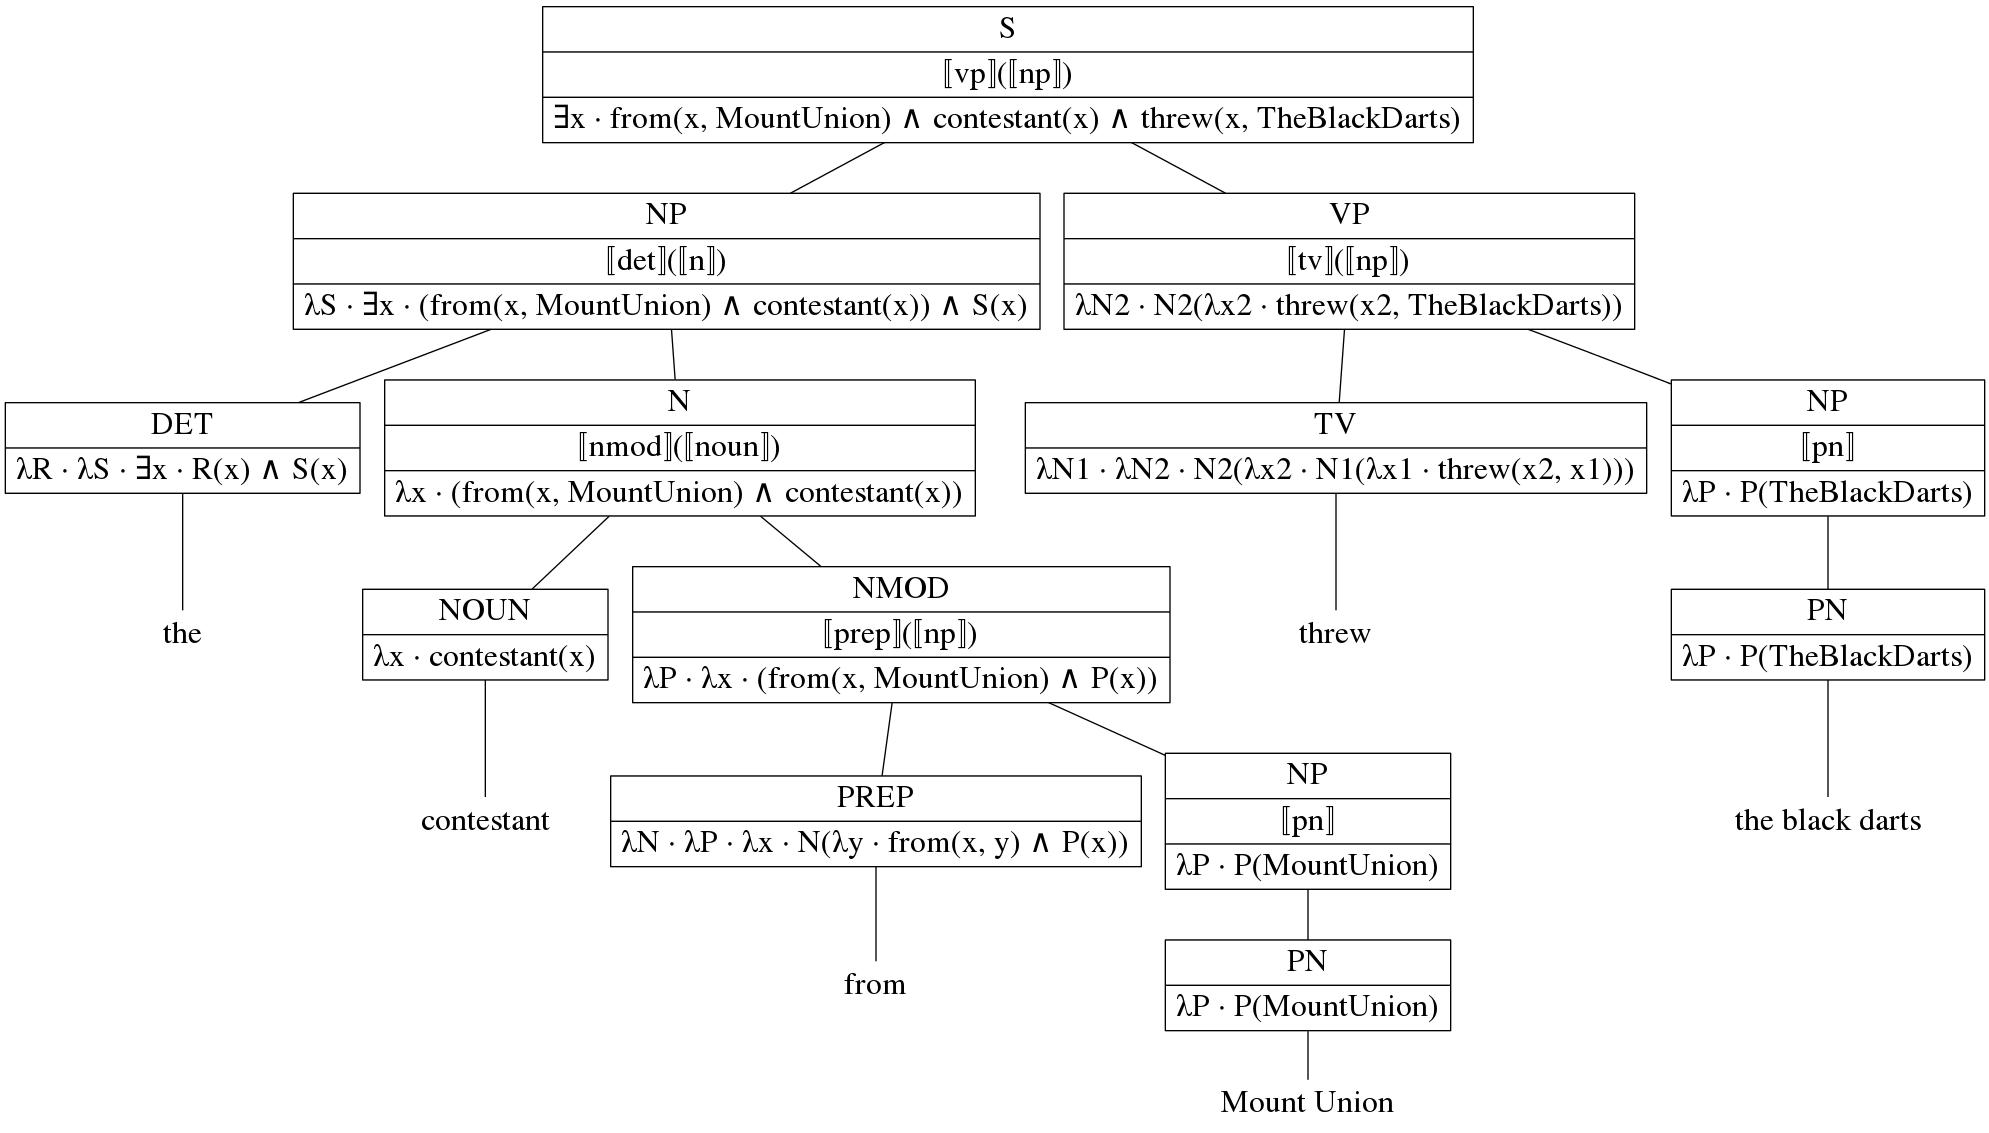
\includegraphics[width=\textwidth]{../../poster/graphviz/tree.jpg}
 Can someone replace this by a picture/schematic overview of the pipeline
 \caption{An overview of the pipeline of \ourtool.}
 \label{fig:overview}
\end{figure*}



\todo{
INCORPORTATE TEH FOLLOWING IN THE PAPER (Jens's description)}

\begin{verbatim}
0. Input
1. POS-tagger
2. POS-rewriter
3. Blackburn \& Bos
4. Transformer to IDP
5. IDP Lua Code
6. Glue code
7. Visualization
\end{verbatim}

\todo{
0. Input: take the input of the puzzle with the sentences and the different things splitted by type (e.g. \url{https://github.com/bartbog/holygrail/blob/master/data/a_bargain.json})

1. POS-tagger
Input: [0. Input]: the json (the clues)
Output: the POS-tags
This is a standard POS-tagger that will take the sentences from [0. Input] and will tag the different words with their Part of Speech tag

2. POS-rewriter
Input: [0. Input]: the json, [1. POS-tagger]: the POS-tags
Output: (A prolog fact with) the rewritten sentences and the problem-specific lexicon
Based on these POS-tags, the POS-rewriter will rewrite some sentences to better match the grammar used in [3. Blackburn \& Bos]. It will also derive the problem specific lexicon.

3. (Adapted) Blackburn \& Bos
Input: [2. POS-rewriter]: the prolog fact with the rewritten sentences and the problem-specific lexicon
Static input (same for all the problems): the grammar that was derived during my thesis, the semantincs of a word-type (e.g. a verb has meaning X), the semantics of a grammar rule (how to combine the meaning of the words in case those words appear as in the grammar rule). Some of these semantics were provided by Blackburn \& Bos, some were added because they were logic puzzle specific. 
E.g. a sentence of the form "Of X and Y, one A and the other B" is defined in \url{https://github.com/bartbog/holygrail/blob/master/bos/myGrammarSemantics.pl#L33} and \url{https://github.com/bartbog/holygrail/blob/master/bos/myGrammar.pl#L91-L100} and is logic puzzle specific
Output: 
 - The First Order Logic representation of all the sentences
 - (Because it's adapted to have types): The types of all the words in the sentences

Blackburn \& Bos is a general framework with 4 inputs: lexicon, grammar, semantics for the lexicon (per word SORT, not per word!), semantics for the grammar. It works by combining the semantics of the words in the way that the semantics of the grammar specifies. It uses Discourse Representation Theory (DRT) for this because this captures quantors way better + it would work across sentences (not used in logic puzzles but this could capture the "He" in "Bart went jogging. He is tired" as "Bart"). The framework also provides a way to translate the DRT to FOL.

Because I adapted the framework, we also get a type for every word. E.g. for "Bart works in Brussels", it knows the subject of "works in" needs to be of the same type as "Bart" and the object of the same type as "Brussels". 

4. Transformer to IDP:
Input: Ouputs of [3. Blackburn \& Bos], MANUAL: the range of values for the numeric types.
Output: IDP translation of all the knowledge about the puzzle including:
- Typed FOL of all the sentences in the puzzle
- relations between the different predicate in the puzzle
- Typed FOL vocabulary
- (Some problem-specific lua code, but this is just glue)

A lot of this step is just glue to translate the FOL to IDP syntax. This step also does the following however:
- It unifies the different types (across sentences). E.g. "Bart works in Brussels" and "Jens works in Leuven", it will know that Jens and Bart need to be of the same type as the subjects of "works in" need to be off the same type (similar to all other verbs). 
- It detects synonyms (based on types) and add axioms to guarantee these are respected
- It adds some rules for transitive and reflexive relations (problem-specific but based on types!)
- It adds Logigram bijection axioms (not based on types)

This step still requires the range of values for the numeric types, all other questions can be eliminated in case the problem-specific lexicon mentions which ppn's are of the same type.

5. IDP Lua Code
Input: IDP Theory with the axioms + IDP Theory per sentence + Vocabulary
Output: Step-wise solution of the problem (including dependencies and sentence used to derive)

It tries to see what must hold given a theory and the axioms and a minimal set of things already known to be true/false. I hope Bart can give more info

6. Glue Code
(Not really important)
This just transforms the json from Bart a bit and saves it somewhere: \url{https://github.com/bartbog/holygrail/blob/master/bos/output/p2_types.output.json}
There is also a json from step 4 that lists all instances of all the types (grouped by type): \url{https://github.com/bartbog/holygrail/blob/master/bos/output/p2_types.voc.json}
-> It used the types for the latter but this could probably also be generated based on the input json

7. Visualization
Input: The 2 json's from above
Output: A step-wise visualization
}
% \end{verbatim}
